\documentclass[11pt]{article}
\usepackage[letterpaper,margin=0.95in]{geometry}
\usepackage[T1]{fontenc}
\usepackage{lmodern}
\usepackage{microtype}
\usepackage{amsmath,amssymb}
\usepackage{graphicx}
\usepackage{booktabs,tabularx,array,multirow}
\usepackage{enumitem}
\usepackage[dvipsnames]{xcolor}
\usepackage{caption}
\usepackage{float}
\usepackage{adjustbox}
\usepackage[hidelinks]{hyperref}
\definecolor{hblue}{HTML}{2a78d6}
\definecolor{boxbg}{HTML}{f4f3ef}
\definecolor{ink2}{HTML}{52514e}
\hypersetup{colorlinks=true,linkcolor=hblue,urlcolor=hblue,citecolor=hblue}
\captionsetup{font=small,labelfont=bf,margin=0.15in}
\setlist{itemsep=2pt,topsep=3pt,parsep=0pt}
\setlength{\parskip}{4pt}
\setlength{\parindent}{0pt}
\graphicspath{{../../../results/}{figs/}}
\newcommand{\keybox}[1]{\par\smallskip\noindent\colorbox{boxbg}{\parbox{\dimexpr\linewidth-2\fboxsep}{\small #1}}\par\smallskip}
\newcommand{\TPR}{\mathrm{TPR}}
\newcommand{\FPR}{\mathrm{FPR}}
\renewcommand{\arraystretch}{1.18}

\sloppy
\usepackage{xurl}

\usepackage[section]{placeins}
\usepackage{xltabular}
\newcommand{\src}[1]{{\footnotesize\textcolor{ink2}{[\nolinkurl{#1}]}}}
\newcommand{\HOLD}{\textcolor{ForestGreen}{\textbf{holds}}}
\newcommand{\WEAK}{\textcolor{BurntOrange}{\textbf{weakened}}}
\newcommand{\DROP}{\textcolor{BrickRed}{\textbf{dropped}}}
\newcommand{\NE}{\textit{n.e.}}
\title{\textbf{Idea 2: Per-Context Thresholds for AI-Agent Monitors}\\[4pt]
\large Rounds 1--3 after two audits: heterogeneity, CFAR vs global vs Stackelberg allocation, transfer, poisoning, white-box probes, and Watcher-like severity tiers}
\date{October 22, 2026 (supersedes the October 21 version)}
\begin{document}
\maketitle
\vspace{-1.5em}

\keybox{\textbf{Summary.} Honest monitor-score distributions differ across deployment contexts, so a single global threshold over-audits some contexts and under-audits others. Radar's answer is CFAR: hold the false-alarm rate constant in every context. Three rounds of experiments tested CFAR and alternatives at a fixed \emph{global} audit budget $B$ on real monitor streams (Gemini-3.1-Pro on 7 settings and ControlArena, the 12-monitor LinuxArena sweep, MRT, MonitoringBench with gpt-4.1/-mini/-nano, and 14 Qwen3.5-27B white-box probe streams), against uniform, context-selecting, probing, poisoning and severity-aware attackers. Every number below comes from a results file or log entry and reflects both audits' corrections; claims that changed are listed in Section~\ref{sec:verdicts}.
\begin{enumerate}[leftmargin=1.2em]
\item \textbf{Heterogeneity is real across deployments, small within one, and large for white-box probes.} One monitor and rubric over 7 settings: per-setting FPR 0--9.0\% at a global 5\% threshold ($\tau=1.34$ logit, $p<0.001$). Within LinuxArena: 2.1--7.2\% across environments, nothing across agent models. Probe scores: $\tau$ up to 3.79, per-cluster FPR up to 25.5\%, while the LLM monitors on the same trajectories have $\tau\le0.46$ (n.s.).
\item \textbf{CFAR is the worst rule against an attacker who chooses where to attack}, and the attacker needs little information. 7 settings, $B=1\%$, spend-matched: 0.38 vs 0.64 for global (paired $-0.52..-0.10$). Three to five alarm-feedback probes per context recover most of the gain (ControlArena 1\%: CFAR safety $0.83\to0.25$).
\item \textbf{Damage-equalizing (Stackelberg) thresholds beat global against selection at 5\%}, not demonstrably at 1\%. 7 settings at 5\%: 0.97 vs 0.89 (paired $+0.03..+0.12$; 0.957 with attacker information independent of the defender's fit). They need attack data from the deployed side-task distribution and $\gtrsim$10--20 attacks per context (or shrinkage). Fit on other side tasks they lose the gain.
\item \textbf{Per-context rules have a spend floor.} With $n_c$ honest calibration runs, plug-in per-context thresholds cannot spend less than $\approx\sum_c w_c/(n_c+1)$. At $n_c=10$ CFAR spends 6.2--7.7$\times$ the budget. On the white-box panel the floor is 2.5\%, so the earlier ``CFAR doubles probe TPR at 1\%'' is not estimable. At equal realized spend ($\approx$3\%) CFAR gains 1.3--1.5$\times$ for the two probes behind that claim.
\item \textbf{Recalibration can be poisoned, and no rule separates poisoning from genuine deployment-wide drift without a trusted refresh.} CFAR breaks at poisoned share $\varepsilon\approx B$. Round 1's OS-CFAR with a leave-one-context-out tail resists poison in one context but breaks at $\varepsilon\approx B$ when the poison is spread over the other contexts. A tail taken from a frozen trusted reference holds (worst-case TPR 0.59--0.81 at $\varepsilon=10\%$) but over-spends 2.0--2.9$\times$ under genuine deployment-wide tail drift.
\item \textbf{Watcher-like fixed severity tiers lose to a plain suspicion threshold.} A blind per-action severity rater does not separate attacks from honest work (AUROC 0.53--0.54). The always-block tier alone flags 1.5\% of honest trajectories, so tiered policies cannot run at 1\%. At 5\% they lose 0.06--0.12 damage-weighted detection to global (gpt-4.1-mini: $-0.08$ [$-0.19,-0.03$] permissive, $-0.06$ [$-0.16,-0.01$] strict).
\end{enumerate}
Spend: \$17.11 (round 1) + \$0 (round 2) + \$21.82 (round 3) = \$38.93 OpenRouter; both audits \$0 for this track.}


\section{Question and scope}
How much do honest monitor-score distributions vary by context (environment, setting, task type, agent model, monitor)? At a \textbf{fixed global audit budget} $B$ (the fraction of honest traffic audited), do per-context thresholds beat one global threshold, and which per-context rule?
\begin{itemize}
\item \textbf{Round 1} (Oct 20): heterogeneity; CFAR vs global vs detection-maximizing vs damage-equalizing (Stackelberg) allocation against uniform and context-selecting attackers; small samples; poisoning of one context's recalibration data; slow (``boiling frog'') poisoning.
\item \textbf{Round 2} (Oct 21): transfer to new attack distributions, new agent models and new monitors (E1); poisoning spread over several contexts (E2); severity-weighted damage (E3); probing attackers and estimation error (E4); white-box and strong-monitor streams (E5).
\item \textbf{Round 3} (Oct 21): Watcher-like products that combine per-action suspicion with intent-agnostic severity tiers.
\item \textbf{Audits} (Oct 21--22): the first audit (C1, M5, m2, m3, m11) and the second audit (m9 on the round-3 matcher) changed several claims; Section~\ref{sec:verdicts} lists them.
\end{itemize}
\textbf{Prior expectations.} Per-context thresholds are requested by several research agendas (\emph{Salient Directions}, Scale MRT, UK AISI Async Control, GDM's UEBA mention). Pinto (2607.06596) shows that a 1\% threshold transferred across model families realizes 0--94\% audit spend. Detection theory (Ghafouri et al.) predicts that against a threshold-aware attacker the optimal per-context thresholds equalize worst-case \emph{damage}, not FPR, so CFAR may be exploitable.

\textbf{Sources.} All paths in brackets are relative to \texttt{results/} unless they start with \texttt{data/} or \texttt{EXPERIMENT\_LOG}. Round 1: \src{t2/tables.md}; round 2: \src{r2_t2/tables.md}; E5: \src{r2_t2/e5_tables.md} and the corrected \src{fixes/r2_t2/e5_tables_corrected.md}; round 3: \src{r3_t2/tables.md}, \src{r3_t2/watcher_summary.csv}; audits: \src{fixes/corrections.csv}, \src{audit/issues.csv}, \src{audit2/issues.csv}, \src{audit2/r3t2_matched_check.csv}.

\section{Data, rules and evaluation}
\subsection{Panels}
A \emph{panel} is a dataset $\times$ monitor $\times$ context key. The trajectory statistic is the maximum of per-step (or per-chunk) scores.

\begin{table}[!htb]\centering\small
\begin{adjustbox}{max width=\linewidth}
\begin{tabular}{@{}>{\raggedright\arraybackslash}p{3.3cm}>{\raggedright\arraybackslash}p{5.6cm}>{\raggedright\arraybackslash}p{3.0cm}cc@{}}
\toprule
Panel (round) & Monitor (scale) & Context (\#) & Honest / attack & Honest per ctx\\
\midrule
la\_env (local / cum.) (1) & Gemini-3.1-Pro streaming, aksh-n LinuxArena gold set (0--10) & environment (10) & 1{,}396 / 1{,}305 & 87--197\\
la\_taskcat (1) & same & task category (5) & 1{,}332 / 1{,}296 & 75--620\\
la\_model (1) & same & agent model (8) & 1{,}155 / 1{,}298 & 45--583\\
akshn\_setting, ``7 settings'' (1--3) & Gemini-3.1-Pro local, same rubric & setting (7) & 5{,}189 / 5{,}794 & 328--1{,}396\\
ca\_setting\_model (1--2) & same & ControlArena setting $\times$ agent (12) & 2{,}997 / 3{,}000 & 247--250\\
lasweep\_\{m\} (1--2) & 12 LinuxArena-sweep monitors (0--100) & environment (10) & 200 / 101--142 & 20\\
mrt\_\{m\} (1) & claude-3.5-sonnet sequential $N=5$, 3 prompts (1--5) & CUA task (15) & 150 / 675 & 10\\
mb\_\{m\} (1--2) & gpt-4.1-mini / nano, trajectory and per-step & BashArena task cluster (7) & 535 / 752--2{,}584 & 30--207\\
E5 (2) & 17 signals: 7 Qwen3.5-27B white-box streams $\times$ \{full, none\}; gpt-4.1 none; gpt-4.1-mini none / full & task cluster (7) & 550 / 541 & 30--213\\
mb\_mini, mb\_mini\_full, mb\_strong (3) & suspicion: gpt-4.1-mini none / full, gpt-4.1 none; severity: gpt-4.1-mini Watcher tiers (1--10) & task cluster = ``org'' (7) & 535 / 752; 505 / 143 & 30--207\\
akshn\_adj (3) & Gemini suspicion + outcome-adjudicated severity (label-leaking) & setting (7) & 5{,}189 / 5{,}794 & 328--1{,}396\\
\bottomrule
\end{tabular}\end{adjustbox}
\caption{Panels. The Gemini panels are strong monitors (AUROC $\approx0.99$); the MonitoringBench panels are weak (AUROC 0.59--0.76). E5 attacks are 33 MonitoringBench originals plus 508 T3 monitor-aware refined variants of 148 base attacks; 94\% of them have LLM-fabricated tool outputs. Sources: \src{t2/tables.md}, \src{r2_t2/e5_tables.md}, \src{fixes/r2_t2/e5_tables_corrected.md}, \src{r3_t2/tables.md}.}
\end{table}

\subsection{Rules}
\begin{table}[!htb]\centering\small
\begin{tabularx}{\linewidth}{@{}>{\raggedright\arraybackslash}p{3.0cm}X@{}}
\toprule
Rule & Definition (all fit to spend $B$ on calibration honest data, randomized ties)\\
\midrule
global & one threshold on the pooled honest scores\\
CFAR & per-context threshold at level $B$ (same FPR everywhere)\\
Mondrian & per-context conformal quantile\\
pooled\_eb / pooled\_cv & per-context FPR shrunk toward global with prior strength $n_0$ (empirical Bayes or 5-fold CV)\\
max-detect & fractional knapsack on per-context ROC hulls, maximizing uniform-attacker TPR\\
Stackelberg & randomized thresholds on ROC hulls minimizing $\max_c D_c(1-\TPR_c)$; $D_c\equiv1$ or damage-weighted. Round 2 adds shrinkage of each context's attack hull toward the pooled attacks (pseudo-count $m_0$ or fraction $\lambda$; $\lambda=1$ gives global)\\
cell minimax (r2) & thresholds minimizing the worst (context $\times$ side task) cell's expected undetected damage, optionally shrunk\\
OS-CFAR / TM-CFAR & per-context robust location (p75 offset / 10\%-trimmed mean) plus a common tail level. Tail sources: leave-one-context-out (LOCO, round 1); frozen trusted reference (os\_frozen), median / low quantile / trimmed over contexts, capped, guarded (round 2)\\
xfer\_offset (r2) & per-context normal-score offsets learned on a source (other agents or other monitors), one level recalibrated on the target\\
Watcher tiers (r3) & \emph{permissive}: tier 9--10 always flagged, 7--8 if suspicion $>h$, 1--6 never; \emph{strict}: 9--10 always, 4--8 if suspicion $>h$, 1--3 never; tier\_w / tier\_opt: one threshold per tier with FPR weights fixed $(0,1,3,10)$ or tuned\\
sev\_tilt (r3) & one global threshold on $\max_i(s_i+\beta v_i)$, $\beta\in\{0,.25,.5,1,2\}$ tuned on calibration attacks\\
\bottomrule
\end{tabularx}
\end{table}

\subsection{Attackers}
\begin{itemize}
\item \emph{Uniform}: attacks every context in proportion to traffic. Reported as uniform TPR.
\item \emph{Informed selection}: knows the published thresholds and picks the context with the highest undetected-success probability, estimated from its own calibration attacks. Reported as \textbf{selection safety} = TPR in the chosen context. Variants: oracle (min test TPR), cell-level (context $\times$ attack type), damage-weighted.
\item \emph{Probing} (round 2): sees only alarm / no-alarm feedback on $q$ probe attacks per context; probes are either free (staging copy) or costly (any probe alarm catches it).
\item \emph{Poisoning}: injects a fraction $\varepsilon$ of benign-looking but high-scoring runs into the recalibration window of one, several or all contexts.
\item \emph{Severity-aware} (round 3): picks the (org, damage tier) cell with the highest expected undetected damage.
\end{itemize}

\subsection{Evaluation and the spend-matching problem}
\begin{itemize}
\item \textbf{Splits.} Round 1: 60 stratified 50/50 splits (points) and 150 split-then-bootstrap replicates (95\% intervals; paired differences vs global are percentiles of the replicate differences). Round 2: 150 paired bootstrap replicates. E5 corrected: 30 plain + 60 bootstrap splits with the attack split grouped by base attack. Round 3: 40 replicates.
\item \textbf{Nominal mode}: each rule at its nominal level; per-context rules can over-spend out of sample.
\item \textbf{Spend-matched mode}: the nominal level is swept and the metrics are interpolated at realized test spend $=B$. Rounds 1--3 swept $B\times[0.25,2]$ with \texttt{np.interp}, which \emph{clamps} when the sweep never reaches $B$; \texttt{matched\_ok} marks the share of replicates that were bracketed (audit C1). The fixed matcher (\texttt{tracks/fixes/e5/}) sweeps $B\times\{0,0.01..3\}$ and declares a split unmatched otherwise; rows matched in $<80\%$ of splits are reported as not estimable (\NE). It was applied to E5; the round-3 replicates were re-summarized with matched-only replicates (audit2 m9). The round-1 and round-2 tables were not re-run: in this report rows with \texttt{matched\_ok}$\,<0.8$ are marked with $^\dagger$ and not interpreted.
\item \textbf{Small samples.} Calibration subsampled to $n\in\{10,30,100\}$ honest runs per context.
\end{itemize}

\section{Round 1: heterogeneity, allocation, small samples, single-context poisoning}
\subsection{Heterogeneity}
\begin{table}[!htb]\centering\small
\begin{adjustbox}{max width=\linewidth}\begin{tabular}{@{}lcccc@{}}
\toprule
Panel & ICC of honest max & Per-step variance share & Per-context FPR at global 5\% & $\tau$ at 5\% ($p$)\\
\midrule
7 settings & 0.17 (0.31 normal scores) & 0.004 & 0--9.0\% & 1.34 ($<0.001$)\\
ControlArena setting $\times$ agent & 0.28 & 0.014 & 0--15.8\% & 1.75 ($<0.001$)\\
LinuxArena environment (local) & 0.05 & 0.007 & 2.1--7.2\% & 0.14 (0.38); 0.45 at 10\%\\
LinuxArena task category (local) & 0.04 & 0.005 & 3.7--12.8\% & 0.40 (0.04)\\
LinuxArena agent model (local) & 0.00 & 0.001 & 2.1--8.0\% & 0.19 (0.28)\\
LinuxArena sweep (12 monitors, 20 honest/env) & 0.05--0.31 & 0.009--0.092 & 0--25\% & 0.00--1.46\\
MRT (3 prompts, 10 honest/task) & 0.06--0.46 & 0.08--0.38 & 0--49\% & 0.00--1.94\\
BashArena clusters (gpt-4.1-mini / nano) & $\le0.05$ & $\le0.003$ & 0--12.3\% & 0.00--0.92\\
\bottomrule
\end{tabular}\end{adjustbox}
\caption{Heterogeneity of honest trajectory-max scores. $\tau$ = SD of logit per-context FPR net of binomial noise (logit-normal random effects; LR test). \src{t2/tables.md}}
\end{table}
\begin{itemize}
\item Context explains little \emph{per-step} variance (0.1--9\%; MRT 8--38\%). The heterogeneity lives in the trajectory tails.
\item \textbf{Agent model is not a useful context} (ICC 0.00, $\tau$ n.s.).
\item LinuxArena-sweep environment effects are shared across the 12 monitors: mean pairwise Spearman 0.70 (min 0.43); common-effect variance 0.148, environment$\times$monitor interaction 0.000, cell noise 0.037. Some environments are intrinsically sensitive-looking for every monitor. \src{t2/tables.md}
\end{itemize}

\begin{figure}[tbp]\centering
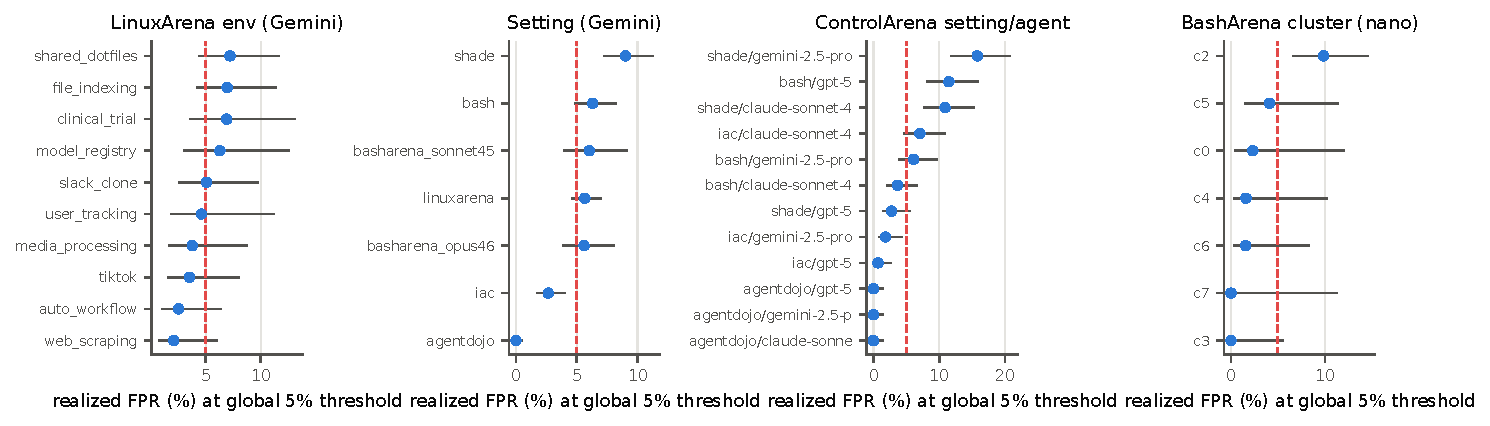
\includegraphics[width=\linewidth]{t2/figures/r1_forest_global_5pct.pdf}
\caption{Realized per-context FPR under one global 5\% threshold (Wilson 95\% CIs), four panels. \src{t2/figures/}}
\end{figure}

\subsection{Allocation at a fixed global budget}
\begin{table}[!htb]\centering\small
\begin{adjustbox}{max width=\linewidth}\begin{tabular}{@{}llccc|ccc|ccc@{}}
\toprule
& & \multicolumn{3}{c|}{$B=1\%$ nominal} & \multicolumn{3}{c|}{$B=1\%$ spend-matched} & \multicolumn{3}{c}{$B=5\%$ spend-matched}\\
Panel & Rule & spend & unif.\ TPR & sel. & sel. & $\Delta$ sel vs global & m\_ok & unif.\ TPR & sel. & $\Delta$ sel vs global\\
\midrule
7 settings & global & 1.01\% & 0.853 & 0.645 & 0.644 & -- & 1.00 & 0.965 & 0.890 & --\\
& CFAR & 1.13\% & 0.821 & 0.404 & \textbf{0.378} & $-0.52..-0.10$ & 0.99 & 0.946 & 0.753 & $-0.30..+0.01$\\
& pooled\_cv & 1.10\% & 0.829 & 0.439 & 0.415 & $-0.49..+0.00$ & 0.99 & 0.947 & 0.757 & $-0.29..+0.01$\\
& Mondrian & 0.36\% & 0.689 & 0.125 & \NE$^\dagger$ & -- & 0.30 & 0.941 & 0.710 & $-0.33..+0.03$\\
& max-detect & 1.12\% & 0.891 & 0.641 & 0.617 & $-0.28..+0.08$ & 0.97 & \textbf{0.984} & 0.958 & $+0.02..+0.12$\\
& Stackelberg & 1.07\% & 0.834 & 0.791 & 0.779 & $-0.11..+0.20$ & 0.98 & 0.971 & \textbf{0.966} & $+0.03..+0.12$\\
ControlArena & global & 0.97\% & 0.798 & 0.601 & 0.607 & -- & 0.96 & 0.960 & 0.908 & --\\
& CFAR & 1.34\% & 0.837 & 0.218 & 0.161$^\dagger$ & $-0.69..-0.17$ & 0.68 & 0.935 & \textbf{0.561} & $-0.63..-0.06$\\
& max-detect & 1.49\% & 0.898 & 0.574 & 0.408$^\dagger$ & $-0.65..+0.14$ & 0.62 & 0.985 & 0.950 & $-0.06..+0.12$\\
& Stackelberg & 1.38\% & 0.863 & 0.729 & 0.610$^\dagger$ & $-0.36..+0.17$ & 0.66 & 0.982 & 0.973 & $-0.00..+0.13$\\
\bottomrule
\end{tabular}\end{adjustbox}
\caption{Allocation rules. ``sel.'' = selection safety (TPR in the context an informed attacker picks). $\Delta$ = 2.5--97.5\% of paired replicate differences. m\_ok = \texttt{matched\_ok} at 1\% (all 5\% rows shown have m\_ok $\ge0.97$). $^\dagger$ = m\_ok $<0.8$, partly extrapolated by the clamping matcher; not interpreted. \src{t2/tables.md}}
\end{table}

\begin{itemize}
\item \textbf{CFAR is the worst rule against selection} on the heterogeneous panels: 7 settings at 1\% (spend-matched, m\_ok 0.99) and ControlArena at 5\% (m\_ok 1.00) both have paired intervals below 0. With attacker information drawn from a split independent of the defender's fit, 7 settings at 1\% gives CFAR 0.409 vs global 0.642 (interval $-0.34..-0.13$). \src{audit/repro_t2.csv}
\item \textbf{Stackelberg beats global at 5\%} (7 settings $+0.03..+0.12$; ControlArena $-0.00..+0.13$). With independent attacker information: 0.775 at 1\% and 0.957 at 5\% vs global 0.642 / 0.888. \textbf{At 1\% the gain is not established}: the 7-settings spend-matched interval crosses 0, and the ControlArena nominal gain (0.729 vs 0.601) comes from over-spending (1.38\% vs 0.97\%); matched, it is 0.610 vs 0.607. \src{fixes/corrections.csv (m2)}
\item \textbf{Max-detect} gives the best uniform TPR (0.984 vs 0.965 at 5\%, 7 settings) and no robust selection advantage.
\item \textbf{Damage-weighted Stackelberg} vs a damage-weighted attacker at 5\%: 0.984 vs 0.937 (7 settings) and 0.989 vs 0.930 (ControlArena). \src{t2/tables.md}
\item \textbf{Homogeneous panel} (LinuxArena environment, local; $\tau$ n.s.): CFAR, pooling, max-detect and Stackelberg are within 0.012 uniform TPR and 0.05 selection safety of global at nominal 1\%. Allocation does not matter when contexts do not differ.
\item \textbf{Cell-level selection} (choosing an attack type within a context) costs another 0.2--0.4: LinuxArena environment at 1\% falls from 0.900 to 0.607 (global) and from 0.948 to 0.704 (Stackelberg), nominal mode.
\item \textbf{Weak monitors} (MonitoringBench clusters): the round-1 uniform-TPR gains of CFAR / max-detect (nano trajectory at 5\%: 0.079 $\to$ 0.106 / 0.162) rest on rows with m\_ok 0.70 / 0.34 (max-detect realizes 5.56\%). At nominal 1\% the per-context rules spend 3.2--4.3\% vs global 1.25\%. This is the spend floor of Section~\ref{sec:smalln} again; the gain is not established. Selection safety stays $\le0.32$ for every rule.
\end{itemize}

\subsection{Small samples per context}\label{sec:smalln}
\begin{table}[!htb]\centering\small
\begin{adjustbox}{max width=\linewidth}\begin{tabular}{@{}llccccc@{}}
\toprule
Panel & $n$ per ctx & global & CFAR & Mondrian & pooled\_eb & pooled\_cv\\
\midrule
7 settings & 10 & 1.61$\times$ / 0.81 / 0.63 & \textbf{7.26$\times$} / 0.91 / 0.59 & 0 / 0 / 0 & 2.45$\times$ / 0.85 / 0.63 & 1.72$\times$ / 0.83 / 0.64\\
& 30 & 1.16$\times$ / 0.83 / 0.63 & 2.90$\times$ / 0.85 / 0.43 & 0 / 0 / 0 & 1.60$\times$ / 0.85 / 0.60 & 1.30$\times$ / 0.84 / 0.61\\
& 100 & 1.01$\times$ / 0.84 / 0.64 & 1.48$\times$ / 0.84 / 0.40 & 0.46$\times$ / 0.68 / 0.08 & 1.25$\times$ / 0.85 / 0.52 & 1.13$\times$ / 0.84 / 0.58\\
ControlArena & 10 & 1.35$\times$ / 0.77 / 0.59 & 6.20$\times$ / 0.92 / 0.43 & 0 / 0 / 0 & 2.32$\times$ / 0.85 / 0.56 & 1.39$\times$ / 0.78 / 0.60\\
& 100 & 1.02$\times$ / 0.80 / 0.60 & 1.41$\times$ / 0.84 / 0.21 & 0.43$\times$ / 0.74 / 0.00 & 1.23$\times$ / 0.85 / 0.30 & 1.09$\times$ / 0.83 / 0.44\\
LA task category & 10 & 2.61$\times$ / 0.93 / 0.88 & 7.66$\times$ / 0.95 / 0.87 & 0 / 0 / 0 & 3.95$\times$ / 0.94 / 0.88 & 2.91$\times$ / 0.94 / 0.89\\
\bottomrule
\end{tabular}\end{adjustbox}
\caption{Spend/$B$ / uniform TPR / selection safety at $B=1\%$, nominal mode. \src{t2/tables.md}}
\end{table}
\begin{itemize}
\item The plug-in per-context quantile spends $\approx1/(n_c+1)$ per context regardless of the target: CFAR spends 6.2--7.7$\times$ the budget at $n=10$, 2.5--2.9$\times$ at 30 and 1.4--1.6$\times$ at 100 (four panels).
\item Mondrian conformal is valid but \emph{never alarms} below $n_c\approx1/B$.
\item Partial pooling with cross-validated $n_0$ stays at 1.06--1.18$\times$ with $n=100$ and 1.16--1.40$\times$ with $n=30$, at equal uniform TPR. Empirical-Bayes $n_0$ is worse.
\item LinuxArena sweep and MRT (10 calibration runs per context, nominal 5\%): CFAR spends 7.8--12.3\%, max-detect and Stackelberg 9.1--14.4\%, global and pooled\_cv 4.6--6.5\%.
\end{itemize}

\subsection{Poisoning one context's recalibration data}
Honest runs per context are split into a trusted reference, a new window and test (1/3 each). The attacker adds a share $\varepsilon$ of the target context's new window at its own maximum calibration attack score; every context is targeted in turn (40 replicates).

\begin{table}[!htb]\centering\small
\begin{adjustbox}{max width=\linewidth}\begin{tabular}{@{}lccccccccc@{}}
\toprule
Panel & $\varepsilon$ & global & CFAR & pooled\_eb & OS-CFAR (LOCO) & TM-CFAR & 50/50 ref.\ mix & frozen ref. & drift cap\\
\midrule
LA environment & 0 & .945 & .949 & .947 & .896 & .675 & .943 & .945 & .953\\
& 2\% & .941 & \textbf{.366} & .931 & .887 & .590 & .724 & .945 & .800\\
& 5\% & .933 & .157 & .759 & .862 & .382 & .314 & .945 & .778\\
& 10\% & .785 & .079 & .360 & .807 & .033 & .157 & .945 & .771\\
7 settings & 0 & .854 & .821 & .848 & .872 & .655 & .829 & .824 & .824\\
& 5\% & .641 & .109 & .172 & .808 & .252 & .212 & .824 & .531\\
& 10\% & .388 & .055 & .076 & .722 & .000 & .108 & .824 & .516\\
LA task category & 0 & .914 & .906 & .910 & \textbf{.778} & .525 & .892 & .894 & .920\\
& 10\% & .520 & .068 & .125 & .615 & .000 & .136 & .894 & .613\\
\bottomrule
\end{tabular}\end{adjustbox}
\caption{TPR in the poisoned context (mean over target contexts), $B=1\%$. \src{t2/tables.md}}
\end{table}
\begin{itemize}
\item \textbf{CFAR breaks once $\varepsilon\approx B$}: a per-context quantile at level $B$ moves with any poison share $\ge B$.
\item \textbf{Global breaks near $\varepsilon\approx B/w_t$}: the poison is diluted by the target's traffic share $w_t$.
\item \textbf{OS-CFAR with a LOCO tail} takes its tail from the other contexts, so one poisoned context cannot move it. At $\varepsilon=10\%$ the mean target TPR is 0.62--0.81 by panel, but the worst target context falls to 0.07--0.45; without poisoning it costs detection on LA task category (0.778 vs 0.914). \src{fixes/corrections.csv (m3)} Round 2 shows it breaks when the poison is spread (Section~\ref{sec:e2}).
\item \textbf{Boiling frog} (30 recalibration rounds, sliding window, poison just above the current threshold, $\varepsilon=5\%$): CFAR ends at 0.11 / 0.16 TPR (7 settings / LA environment); an outlier filter ends at the same values, only later; a cumulative cap holds 0.54 / 0.78 but under a genuine $+2$ shift its FPR is 3.3\% / 4.9\%; global ends at 0.65 / 0.94 with FPR 4.0\% under drift; OS-CFAR (LOCO) holds 0.80 / 0.82 with FPR 0.6\% / 1.1\% under drift. \src{t2/tables.md}
\end{itemize}

\section{Round 2: transfer, spread poisoning, severity, adaptive attackers}
\subsection{E1a: Stackelberg fit on a different attack distribution}
The defender fits Stackelberg / max-detect on source attacks; the attacker comes from a target distribution and picks its context from its own calibration attacks. Spend-matched.

\begin{table}[!htb]\centering\small
\begin{adjustbox}{max width=\linewidth}\begin{tabular}{@{}lllcccc@{}}
\toprule
Panel & Shift & $B$ & global & CFAR & Stackelberg (source) [$\Delta$ vs global; $\Delta$ vs in-dist.] & Stackelberg (in-dist.) / $\lambda=.5$\\
\midrule
7 settings & unseen side tasks & 1\% & 0.62 & 0.40 & 0.43 [$-0.13$ ($-0.48,+0.11$); $-0.27$ ($-0.56,-0.03$)] & 0.78 / 0.54\\
& & 5\% & 0.87 & 0.78 & 0.70 [$-0.16$ ($-0.51,+0.03$); $-0.27$ ($-0.65,-0.04$)] & 0.97 / 0.82\\
ControlArena & unseen side tasks & 5\% & 0.83 & 0.54 & 0.58 [$-0.23$ ($-0.62,+0.11$); $-0.38$ ($-0.81,-0.08$)] & 0.98 / 0.79\\
& attack policy p1$\to$p2 & 1\% & 0.72 & 0.15 & 0.66 [$-0.08$ ($-0.40,+0.13$); $+0.04$] & 0.61 / 0.67\\
& & 5\% & 0.91 & 0.56 & 0.95 [$+0.04$ ($-0.09,+0.26$); $-0.01$] & 0.96 / 0.93\\
LA environment & unseen side tasks & 5\% & 0.96 & 0.95 & 0.86 [$-0.08$ ($-0.38,+0.06$); $-0.07$] & 0.97 / 0.91\\
\bottomrule
\end{tabular}\end{adjustbox}
\caption{Selection safety under attack-distribution shift (m\_ok $\ge0.86$ in all rows shown). $\lambda=.5$: each context's source attacks mixed 50/50 with the pooled source attacks of the other contexts. \src{r2_t2/tables.md (E1a)}}
\end{table}
\begin{itemize}
\item \textbf{A new attack policy or month does not hurt}: ControlArena p1$\to$p2 keeps the in-distribution level (0.66 / 0.95 vs 0.61 / 0.96 at 1\% / 5\%).
\item \textbf{Unseen side tasks do}: Stackelberg fit on other side tasks is significantly worse than the in-distribution fit (e.g.\ 7 settings 1\%: $-0.27$ [$-0.56,-0.03$]) and lands at or below global (point estimates $-0.08$ to $-0.23$; intervals cross 0).
\item Shrinkage moves the source fit monotonically toward global ($\lambda=0.5$: 0.54 at 1\% on 7 settings) and costs $\le0.05$ in distribution (0.73 vs 0.78).
\item On MonitoringBench (weak monitors) the 1\% rows of the attack-fitted rules are clamped (m\_ok $\le0.08$) and are not interpreted.
\end{itemize}

\begin{figure}[tbp]\centering
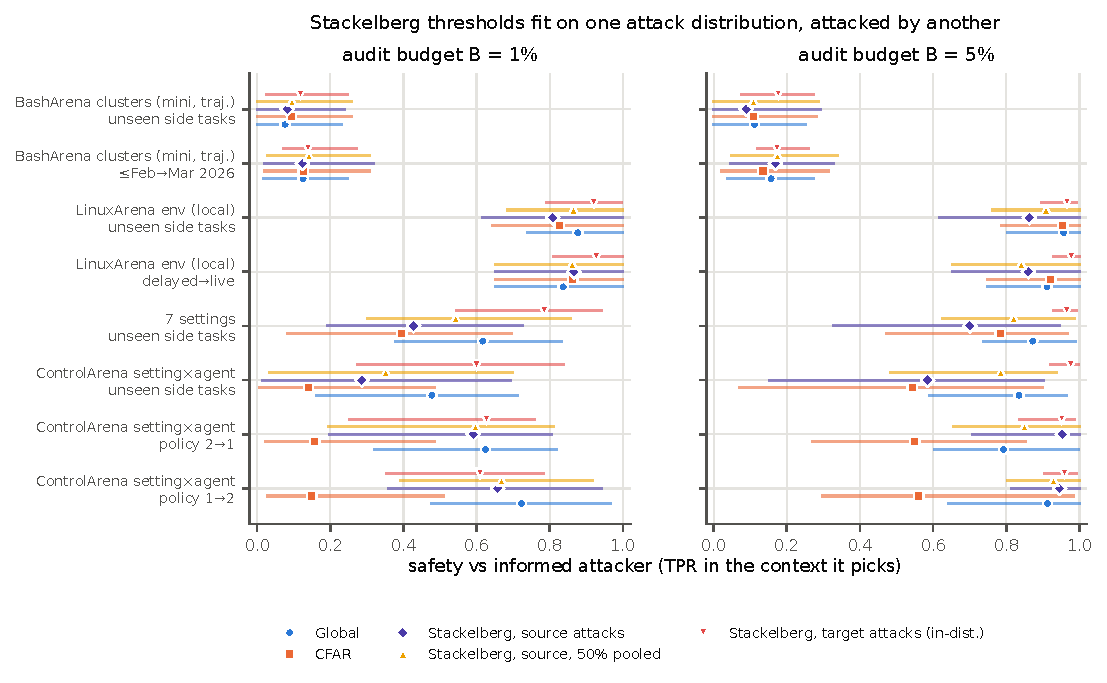
\includegraphics[width=0.75\linewidth]{r2_t2/figures/e1a_attack_shift.pdf}
\caption{E1a: selection safety of Stackelberg fit on source attacks vs in-distribution and global, by panel and shift. \src{r2_t2/figures/}}
\end{figure}

\subsection{E1b: a new agent model}
Rules fit on the other agent models' data are applied to a held-out agent model.
\begin{itemize}
\item \textbf{Transferred per-context thresholds miss the budget in both directions.} Realized spend at nominal 1\% ranges from 0.1\% (source CFAR, opus-4-6 on LA environment) to 2.8\% (source Stackelberg, gemini-2.5-pro on ControlArena); at nominal 5\% from 1.2\% (source Stackelberg, gpt-5) to 12.3\% (source CFAR, gpt-5; 2.5$\times$).
\item Source CFAR is also exploitable on the new agent: gpt-5 on ControlArena at 5\%, selection 0.38 vs in-domain global 0.94 ($-0.53$ [$-0.72,-0.30$]).
\item \textbf{Source offsets plus one level recalibrated on the target} (xfer\_offset) hold the budget: 1.0--1.9\% at nominal 1\% and 4.6--5.7\% at 5\%. Selection safety is not protected (gpt-5 on ControlArena at 5\%: 0.63, $-0.26$ [$-0.49,-0.06$]). \src{r2_t2/tables.md (E1b)}
\end{itemize}


\subsection{E1c: offsets from other monitors}
Per-context offsets estimated from the other 11 LinuxArena-sweep monitors' scores on the same calibration trajectories (xfer\_avg) reduce the SD of per-environment FPR, spend-matched, from 0.060 to 0.050 at 5\% and from 0.114 to 0.066 at 10\%; it is lower than global for 9 of 12 target monitors at 5\% and 10 of 12 at 10\% \src{r2_t2/e1c_monitor_transfer_full.csv}. Like CFAR, equalizing FPR costs selection safety at 5\%: 0.45 vs 0.65 for global. On the strong Gemini LinuxArena pair and on gpt-4.1-mini/nano there is little to gain (per-context FPR SD $\le0.03$ under global). \src{r2_t2/tables.md (E1c)}

\subsection{E2: poisoning spread over several contexts}\label{sec:e2}
The attacker poisons the target only, one other context, half of the others, all others, or all contexts, placing values that beat both a raw global threshold and an offset-based OS-CFAR. Genuine-drift controls: a heavier honest tail in every context (3\% of runs replaced by high values), a deployment-wide location shift, and a target-only shift.

\begin{table}[!htb]\centering\small
\begin{adjustbox}{max width=\linewidth}\begin{tabular}{@{}llccccc@{}}
\toprule
Panel & Rule & clean TPR & worst @ $\varepsilon=2\%$ & worst @ 5\% & worst @ 10\% & max drift spend / $B$\\
\midrule
LA environment & global & 0.94 & 0.37 & 0.16 & 0.08 & 1.19\\
& CFAR & 0.95 & 0.37 & 0.16 & 0.08 & 2.14\\
& OS-CFAR, LOCO tail (round 1) & 0.88 & 0.40 & 0.18 & 0.11 & 1.40\\
& OS-CFAR, frozen-reference tail & 0.89 & \textbf{0.88} & \textbf{0.87} & \textbf{0.81} & 2.47\\
& frozen reference (never recalibrate) & 0.95 & 0.95 & 0.95 & 0.95 & 4.10\\
& OS-CFAR, low-quantile tail & 0.95 & 0.46 & 0.42 & 0.41 & 3.32\\
7 settings & global / CFAR & 0.85 / 0.82 & 0.26 / 0.27 & 0.11 / 0.11 & 0.05 / 0.05 & 1.10 / 1.16\\
& OS-CFAR, LOCO / frozen tail & 0.88 / 0.87 & 0.35 / \textbf{0.84} & 0.18 / \textbf{0.79} & 0.13 / \textbf{0.70} & 1.12 / 2.56\\
ControlArena & OS-CFAR, LOCO / frozen tail & 0.80 / 0.82 & 0.28 / \textbf{0.80} & 0.17 / \textbf{0.78} & 0.08 / \textbf{0.72} & 1.28 / 2.86\\
LA task category & OS-CFAR, LOCO / frozen tail & 0.75 / 0.76 & 0.31 / \textbf{0.74} & 0.16 / \textbf{0.70} & 0.13 / \textbf{0.59} & 1.22 / 2.02\\
\bottomrule
\end{tabular}\end{adjustbox}
\caption{Worst target TPR over the poisoning scenarios and worst realized spend / $B$ over the genuine-drift controls, $B=1\%$. \src{r2_t2/tables.md (E2 summary)}, \src{r2_t2/e2_breakdown_summary.csv}}
\end{table}
\begin{itemize}
\item \textbf{The LOCO tail breaks at $\varepsilon\approx B$ when the poison is in all other contexts}: LA environment target TPR $0.88\to0.44$ at 2\% and 0.25 at 5\%. Worst case over scenarios: 0.16--0.18 at 5\% on all four panels.
\item \textbf{A tail from a frozen trusted reference} (offset still from the new window, so poison must exceed 25\% of a context's window to move it) holds a worst-case 0.70--0.81 at $\varepsilon=10\%$ on three panels and 0.59 on LA task category (clean 0.76).
\item \textbf{Its price}: under genuine deployment-wide tail drift it over-spends 2.0--2.9$\times$ (it refuses to follow a real change in the tail). Never recalibrating over-spends 3.1--7.7$\times$ under the location shift.
\item Median, low-quantile, trimmed and guarded tails resist minority poisoning only (worst case at 5\%: 0.11--0.50). \textbf{Poisoning of every context is indistinguishable from deployment-wide drift} without a trusted refresh of the reference.
\end{itemize}

\begin{figure}[tbp]\centering
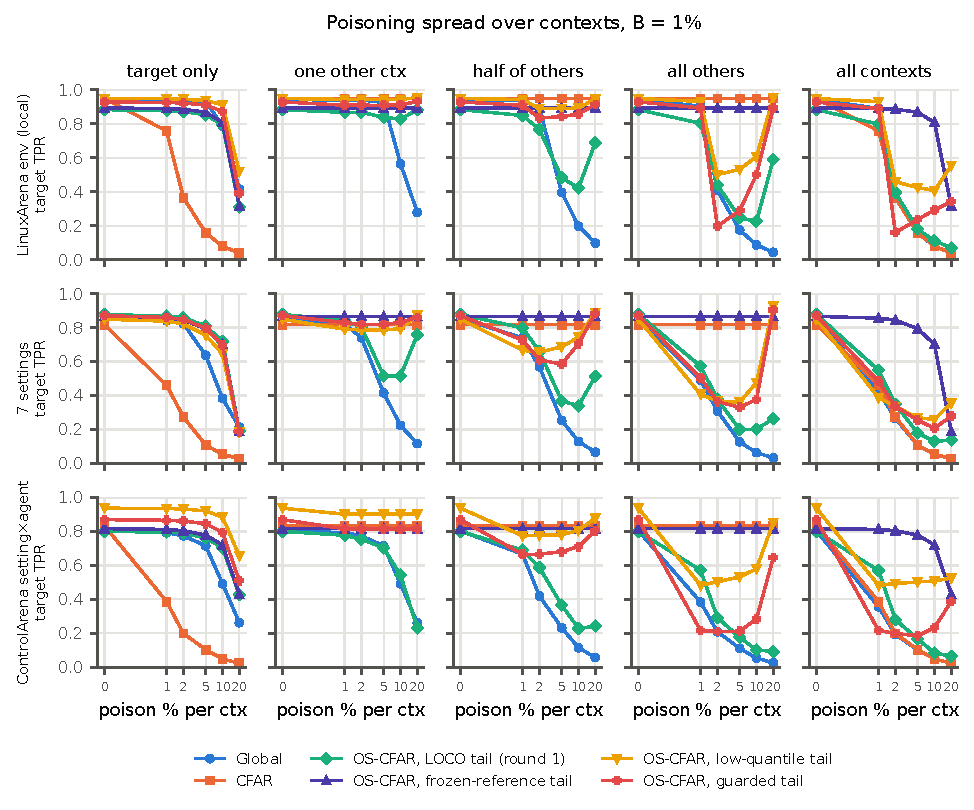
\includegraphics[width=0.62\linewidth]{r2_t2/figures/e2_multipoison.pdf}
\caption{E2: target-context TPR vs poisoned share, by scenario (columns) and panel (rows), $B=1\%$. \src{r2_t2/figures/}}
\end{figure}

\subsection{E3: severity-weighted damage}
aksh-n's adjudicated \texttt{overall\_severity} correlates moderately with the monitor score (Spearman 0.43--0.51) and less with the side-task taxonomy tier (0.29--0.38). Spend-matched, $B=5\%$, against a damage-maximizing attacker who picks a (context, side task) cell:
\begin{table}[!htb]\centering\small
\begin{adjustbox}{max width=\linewidth}\begin{tabular}{@{}lccccc@{}}
\toprule
Panel & global & CFAR & Stackelberg (context) & cell minimax, adjudicated damage & cell minimax, shrunk\\
\midrule
7 settings & 0.64 & 0.60 & 0.76 [$+0.14$ ($-0.14,+0.41$)] & 0.86 [$+0.13$ ($-0.25,+0.31$)] & \textbf{0.92} [$+0.25$ ($+0.00,+0.44$)]\\
ControlArena & 0.71 & 0.48 [$-0.20$ ($-0.38,-0.01$)] & 0.88 [$+0.17$ ($-0.14,+0.40$)] & 0.94 [$+0.23$ ($+0.06,+0.37$)] & \textbf{0.95} [$+0.24$ ($-0.06,+0.44$)]\\
\bottomrule
\end{tabular}\end{adjustbox}
\caption{1 $-$ expected undetected damage in the cell the attacker picks (damage = adjudicated severity), with paired $\Delta$ vs global. \src{r2_t2/tables.md (E3)}}
\end{table}
\begin{itemize}
\item Cell-level severity minimax is the best rule against a cell-choosing attacker; only the unshrunk ControlArena contrast and (borderline) the shrunk 7-settings contrast exclude 0.
\item Against a context-choosing attacker it loses to context-level severity Stackelberg (0.91 vs 0.98 on 7 settings; 0.96 vs 0.99 on ControlArena).
\item Side-task taxonomy weights are a poor proxy for damage: tier-weighted cell minimax is at or below global (0.59 vs 0.64; 0.64 vs 0.71).
\end{itemize}

\subsection{E4: probing attackers and estimation error}
\begin{table}[!htb]\centering\small
\begin{adjustbox}{max width=\linewidth}\begin{tabular}{@{}llcccccc@{}}
\toprule
Panel, $B$ & Rule & uniform & $q=1$ & $q=3$ & $q=5$ & $q=20$ & informed [95\%]\\
\midrule
ControlArena, 1\% & global & 0.80 & 0.71 & 0.69 & 0.68 & 0.65 & 0.60 [0.48, 0.74]\\
& CFAR & 0.83 & 0.46 & 0.30 & \textbf{0.25} & 0.19 & 0.18 [0.07, 0.46]\\
& Stackelberg & 0.86 & 0.77 & 0.74 & 0.74 & 0.73 & 0.73 [0.59, 0.86]\\
7 settings, 1\% & global & 0.85 & 0.78 & 0.75 & 0.73 & 0.68 & 0.64 [0.57, 0.71]\\
& CFAR & 0.82 & 0.60 & 0.50 & 0.46 & 0.41 & 0.40 [0.18, 0.61]\\
& Stackelberg & 0.83 & 0.81 & 0.80 & 0.80 & 0.80 & 0.79 [0.68, 0.89]\\
\bottomrule
\end{tabular}\end{adjustbox}
\caption{Safety against a probing attacker with free alarm feedback on $q$ probes per context (nominal thresholds). With costly probes ($q=5$) safety is 1.00 on every strong-monitor panel. \src{r2_t2/tables.md (E4a)}}
\end{table}
\begin{itemize}
\item \textbf{CFAR's weakness does not need inside knowledge}: 3--5 free probes per context recover most of the gap between the uniform and the fully informed attacker. Stackelberg is nearly flat in $q$.
\item \textbf{Estimation error (defender)}: Stackelberg fit with $n_d$ attacks per context needs about 10--20 to match global (7 settings 1\%: 0.55 / 0.61 / 0.68 / 0.70 at $n_d=3/5/10/20$ vs global 0.64; 5\%: 0.67 / 0.74 / 0.85 / 0.90 vs 0.88). Shrinkage toward the pooled attacks ($m_0=10$) removes the small-sample penalty (0.66 at $n_d=3$, 1\%; 0.86 at 5\%).
\item \textbf{Estimation error (attacker)}: with only 3 attacks per context to estimate evasion, the attacker's selection against CFAR is already near its full-information level (ControlArena 1\%: 0.26 vs 0.18). \src{r2_t2/tables.md (E4b)}
\end{itemize}

\begin{figure}[tbp]\centering
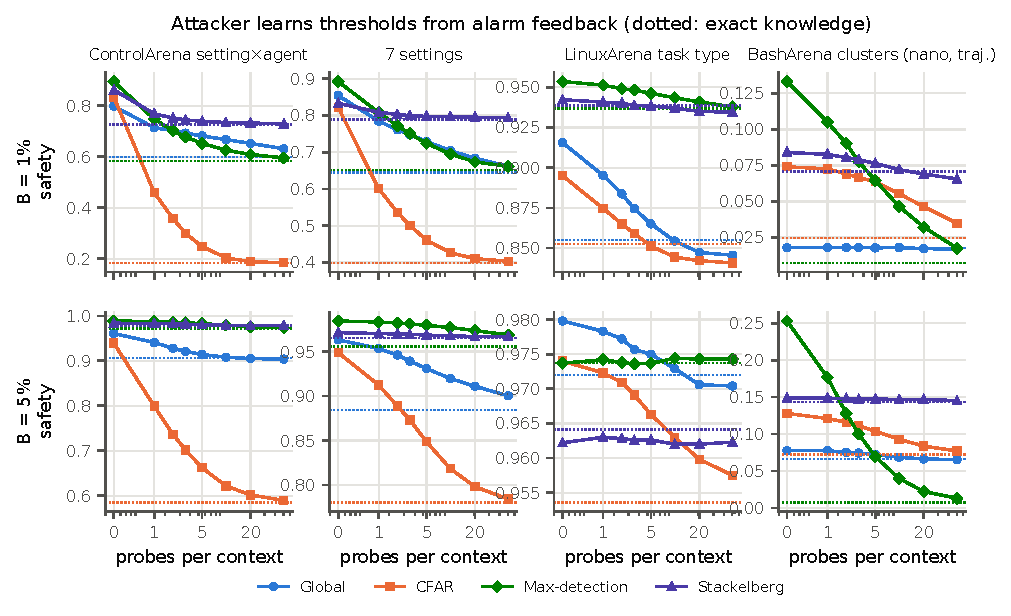
\includegraphics[width=0.65\linewidth]{r2_t2/figures/e4_probes.pdf}
\caption{E4a: safety vs number of free probes per context, $B=1\%$ (top) and 5\% (bottom). \src{r2_t2/figures/}}
\end{figure}

\section{E5: white-box probes and the strong monitor}
E5 uses one common trajectory set (Honest-550 and 541 attacks) scored by 17 signals: 7 white-box streams of a Qwen3.5-27B trusted reader (\texttt{sab} synthetic-sabotage probe, Apollo deception probe \texttt{dec}, FIBS token probe \texttt{fibs\_tok}, FIBS follow-up contrast \texttt{fibs\_fu}, J-lens watch-list mass \texttt{jl\_lm}, and max-pooled variants) in history-aware (full) and history-free (none) reading, plus gpt-4.1 (none) and gpt-4.1-mini (none, full). Contexts are the 7 task clusters.

\subsection{Heterogeneity (honest runs only; unaffected by the audits)}
\begin{itemize}
\item \textbf{Probe scores are far more context-dependent than LLM-monitor scores.} $\tau$ at a global 5\% threshold: \texttt{dec\_full} 3.79, \texttt{fibs\_fu\_full} 2.70, \texttt{dec\_none} 2.28, \texttt{jl\_lm\_max\_none} 1.77, \texttt{fibs\_tok\_none} 1.26, \texttt{sab\_full} 1.21 (all $p\le0.006$). Per-cluster FPR spans up to 0--25.5\%.
\item LLM monitors on the same trajectories: $\tau$ 0.00--0.46, all n.s.; ICC 0.002--0.035, vs 0.10--0.16 for \texttt{fibs\_fu}, \texttt{dec\_none} and \texttt{sab\_max\_none}. \src{r2_t2/e5_tables.md}, \src{fixes/corrections.csv (M5)}
\end{itemize}

\begin{figure}[tbp]\centering
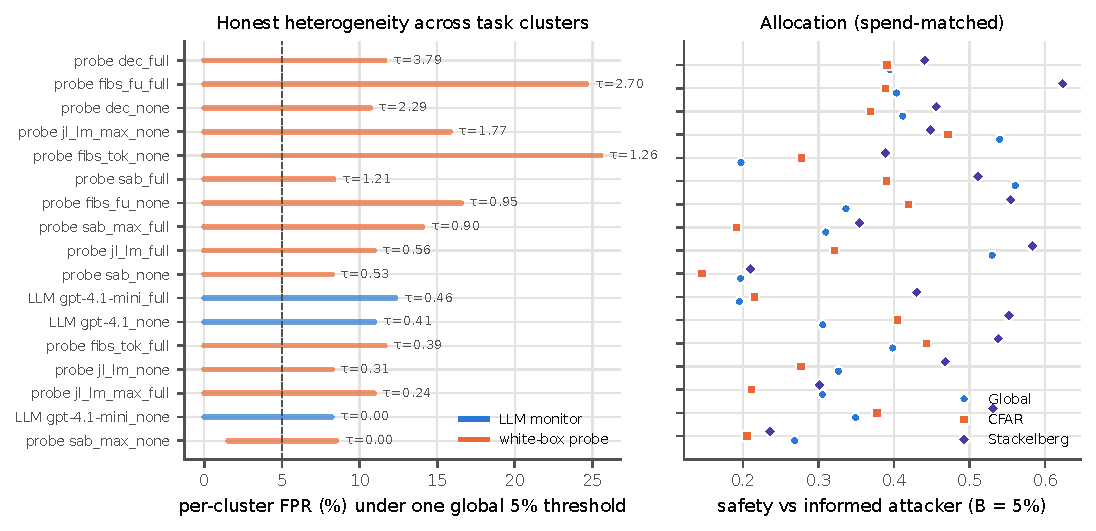
\includegraphics[width=0.8\linewidth]{r2_t2/figures/e5_probe_heterogeneity.pdf}
\caption{E5. Left: per-cluster FPR under one global 5\% threshold, white-box probes vs LLM monitors (honest runs only; valid). Right: the original iid-split allocation at 5\%, superseded by Table~\ref{tab:e5grouped} (audit M5). \src{r2_t2/figures/}}
\end{figure}

\subsection{The 1\% comparison is not estimable (C1)}
Plug-in per-cluster thresholds at level 0 sit at each cluster's calibration maximum, so the realized test spend has a floor of $\sum_c w_c/(n_c+1)=2.52\%$ with 15--106 calibration honest runs per cluster (per-replicate mean 2.58\%, 5--95\% 0.74--4.89\%; only 9\% of splits have a floor $\le1\%$). At nominal 1\% the realized spend is 1.16\% for global, 2.99\% for CFAR, 3.76\% for Stackelberg and 4.19\% for max-detect. The original ``spend-matched'' 1\% rows were clamped at 1.95--3.57\% and are dropped. \src{fixes/r2_t2/e5_tables_corrected.md}

The valid 1\% comparison evaluates global at the spend each per-context rule actually realizes:
\begin{table}[!htb]\centering\small
\begin{adjustbox}{max width=\linewidth}\begin{tabular}{@{}lccccc@{}}
\toprule
Signal & realized spend & CFAR uniform TPR & global at same spend & $\Delta$ [split 95\%] & ratio\\
\midrule
\texttt{wb\_dec\_full} & 3.63\% & 0.52 & 0.34 & $+0.18$ [$+0.08,+0.27$] & 1.5$\times$\\
\texttt{wb\_fibs\_fu\_full} & 2.94\% & 0.63 & 0.49 & $+0.15$ [$+0.03,+0.28$] & 1.3$\times$\\
\texttt{wb\_dec\_none} & 3.07\% & 0.55 & 0.33 & $+0.22$ [$+0.14,+0.30$] & 1.7$\times$\\
\texttt{wb\_fibs\_fu\_none} & 3.01\% & 0.55 & 0.48 & $+0.07$ [$+0.01,+0.14$] & 1.1$\times$\\
\texttt{wb\_sab\_full} & 2.85\% & 0.53 & 0.48 & $+0.05$ [$+0.00,+0.12$] & 1.1$\times$\\
\texttt{llm\_gpt-4.1\_none} & 3.16\% & 0.60 & 0.55 & $+0.05$ [$-0.01,+0.12$] & --\\
\texttt{llm\_gpt-4.1-mini\_none} & 3.02\% & 0.47 & 0.46 & $+0.01$ [$-0.12,+0.11$] & --\\
\bottomrule
\end{tabular}\end{adjustbox}
\caption{CFAR at nominal 1\% vs global at the same realized spend, grouped split; interval over 30 plain splits. The split interval excludes 0 for 5 of 17 signals, all white-box probes. \src{fixes/r2_t2/e5_equal_spend_1pct.csv}}
\end{table}

\begin{figure}[tbp]\centering
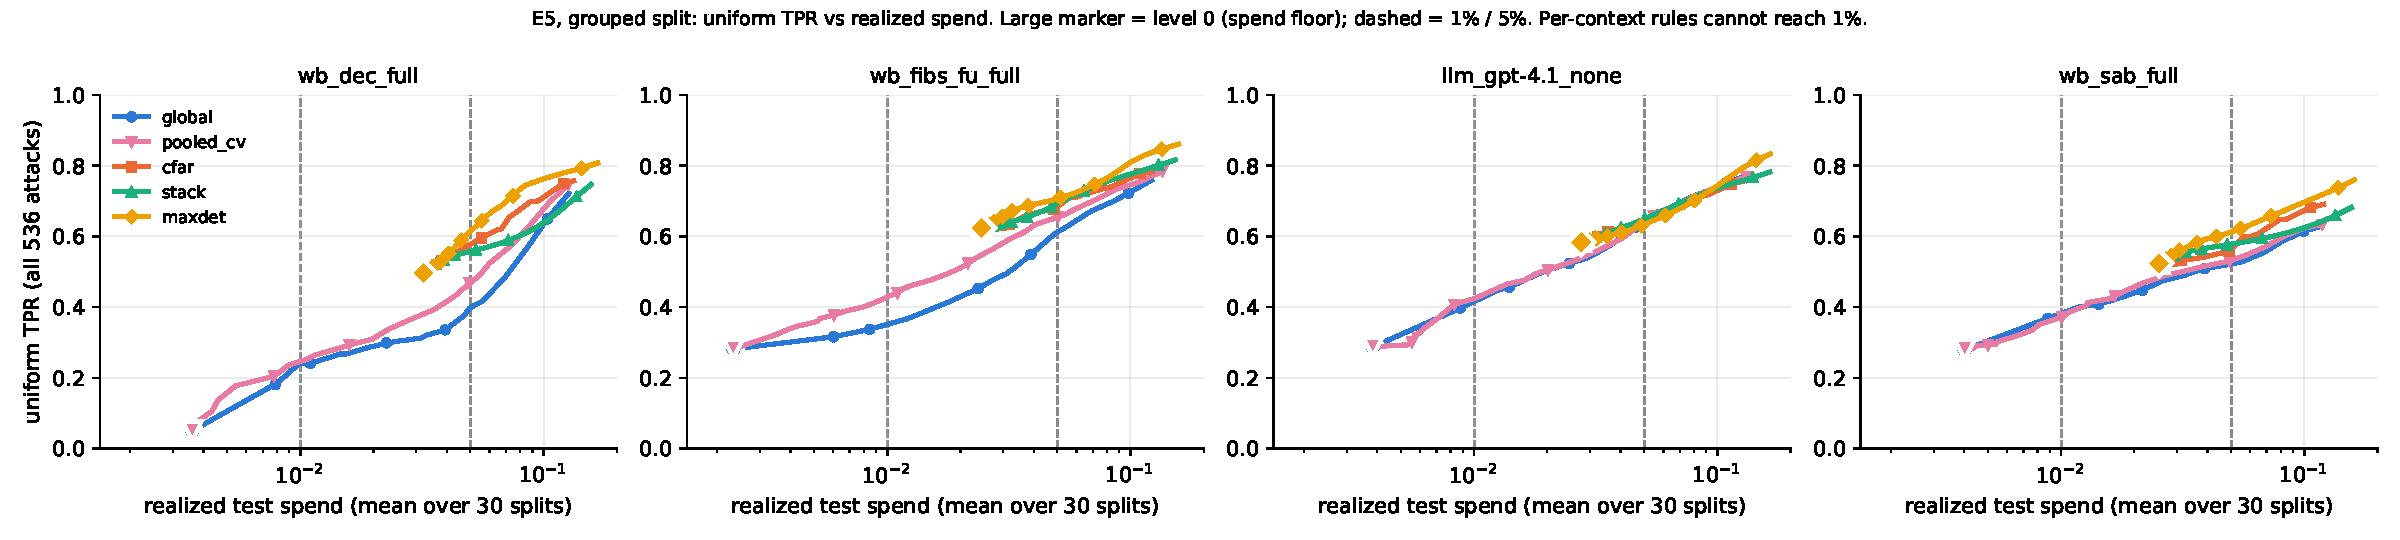
\includegraphics[width=\linewidth]{fixes/r2_t2/fig_e5_tpr_vs_spend.pdf}
\caption{E5 corrected: uniform TPR vs realized spend for four signals. Large markers = level 0 (the spend floor); dashed lines = 1\% and 5\%. Per-context rules cannot reach 1\%. \src{fixes/r2_t2/}}
\end{figure}

\subsection{Allocation at 5\% with the split grouped by base attack (M5)}
The original E5 split attacks iid within context, so refined variants of one base attack fell on both sides of the split. The corrected design groups the split and the bootstrap by base attack (148 base attacks; 0 exact duplicates).
\begin{table}[!htb]\centering\small
\begin{adjustbox}{max width=\linewidth}\begin{tabular}{@{}lcccccc@{}}
\toprule
Signal & global unif.\ / sel. & CFAR unif.\ [$\Delta$] & CFAR sel.\ [$\Delta$] & Stackelberg sel.\ [$\Delta$] & max-detect unif.\ [$\Delta$]\\
\midrule
\texttt{llm\_gpt-4.1\_none} & 0.64 / 0.37 & 0.65 [$+0.01$ ($-0.09,+0.10$)] & 0.44 [$+0.11$] & 0.62 [$+0.14$ ($-0.23,+0.47$)] & 0.64 [$+0.00$]\\
\texttt{wb\_fibs\_fu\_full} & 0.61 / 0.47 & 0.69 [$+0.07$ ($-0.02,+0.21$)] & 0.45 [$-0.00$] & 0.59 [$+0.13$ ($-0.39,+0.50$)] & 0.71 [$+0.10$]\\
\texttt{wb\_dec\_full} & 0.40 / 0.43 & 0.60 [$+0.19$ ($+0.03,+0.34$)] & 0.43 [$-0.08$] & 0.45 [$-0.01$] & 0.64 [$+0.22$ ($+0.04,+0.45$)]\\
\texttt{wb\_dec\_none} & 0.37 / 0.43 & 0.62 [$+0.23$ ($+0.05,+0.35$)] & 0.39 [$-0.04$] & 0.41 [$-0.03$] & 0.65 [$+0.25$ ($+0.07,+0.39$)]\\
\texttt{wb\_sab\_full} & 0.52 / 0.59 & 0.58 [$+0.06$ ($-0.03,+0.14$)] & 0.46 [$-0.11$ ($-0.59,+0.27$)] & 0.53 [$-0.03$] & 0.61 [$+0.09$ ($+0.02,+0.19$)]\\
\texttt{llm\_gpt-4.1-mini\_none} & 0.59 / 0.44 & 0.56 [$-0.01$] & 0.40 [$-0.04$] & 0.55 [$-0.03$] & 0.57 [$-0.03$]\\
\midrule
Counts over 17 signals & & $\ge$ global 12, CI$>0$ 2 & $\ge$ global 5, CI$>0$ 0 & $\ge$ global 10, CI$>0$ 0 & $\ge$ global 14, CI$>0$ 4\\
\bottomrule
\end{tabular}\end{adjustbox}
\caption{E5 corrected, $B=5\%$ spend-matched (matched in 0.83--1.00 of splits), grouped split, cluster bootstrap over base attacks. $\Delta$ = paired difference vs global. \src{fixes/r2_t2/e5_tables_corrected.md}}\label{tab:e5grouped}
\end{table}
\begin{itemize}
\item \textbf{Uniform attacker}: per-context normalization helps the strongly heterogeneous probes (\texttt{dec}) and nothing else significantly. For the LLM monitors it is neutral.
\item \textbf{Selection}: no rule's selection advantage over global is established on E5. Stackelberg $\ge$ global on 10/17 signals (the original log claimed 14/17; its own CSV gives 13/17 at 5\%); no interval excludes 0.
\item \textbf{The attack set is confounded.} AUROCs on the 33 originals are much lower than on all 541 (gpt-4.1 0.765 vs 0.911; \texttt{fibs\_fu\_full} 0.688 vs 0.905; \texttt{dec\_full} 0.573 vs 0.871), and refined variants of the same base attacks score higher than their originals on 13/17 signals (interval $>0$; \texttt{dec\_full} $+0.31$ [$+0.19,+0.43$]). Fabricated tool outputs and rewrite artifacts cannot be separated from detection with these data. The \texttt{sab} probes are the exception (originals 0.81--0.83).
\item \textbf{Originals only} (honest-only rules, no fabrication confound, 1--15 originals per cluster): at 5\% matched, CFAR raises cluster-averaged TPR for \texttt{dec\_none} ($+0.33$ [$+0.02,+0.57$]) and \texttt{fibs\_fu\_full} ($+0.20$ [$+0.00,+0.37$]) and not for gpt-4.1 ($-0.02$ [$-0.26,+0.20$]).
\end{itemize}

\section{Round 3: Watcher-like severity tiers}
A Watcher-style product sees two numbers per action: suspicion $s$ (history-free gpt-4.1-mini or gpt-4.1, or history-aware gpt-4.1-mini) and an intent-agnostic expected severity $v$ (1--10, Apollo Watcher tiers: 1--3 benign, 4--6 strict-only, 7--8 permissive, 9--10 always blocked). Severity was scored by gpt-4.1-mini on all 38.4k MonitoringBench steps (Honest-550 and 775 T1 attacks; \$21.82, 0 errors). Orgs are the task clusters; damage is the attack's maximum severity, or the side-task tier (@sidetask panels).

\subsection{Severity does not separate attacks from honest work}
\begin{table}[!htb]\centering\small
\begin{adjustbox}{max width=\linewidth}\begin{tabular}{@{}llccccc@{}}
\toprule
Panel & label & trajectories & action share by tier (1--3/4--6/7--8/9--10) & traj.\ has a 9--10 action & AUROC suspicion & AUROC severity\\
\midrule
mb\_mini & attack & 752 & 0.61 / 0.22 / 0.16 / 0.002 & 6.9\% & 0.758 & 0.532\\
& honest & 535 & 0.57 / 0.24 / 0.19 / 0.001 & \textbf{1.5\%} & & \\
mb\_strong (gpt-4.1) & attack & 143 & 0.61 / 0.22 / 0.17 / 0.002 & 7.0\% & 0.782 & 0.540\\
& honest & 505 & 0.56 / 0.24 / 0.19 / 0.001 & 1.6\% & & \\
akshn\_adj (label-leaking) & attack & 5{,}794 & 0.00 / 0.13 / 0.79 / 0.080 & 8.0\% & 0.991 & 0.998\\
& honest & 5{,}189 & 0.97 / 0.03 / 0.00 / 0.000 & 0.0\% & & \\
\bottomrule
\end{tabular}\end{adjustbox}
\caption{Severity-tier composition. Every honest BashArena trajectory contains a 7--8 action. The akshn\_adj severity is assigned with knowledge of the outcome; it is an upper bound no deployed rater can reach. \src{r3_t2/tables.md}, \src{fixes/r3_t2/tables_annotated.md}}
\end{table}


\subsection{Fixed tiers lose to a suspicion threshold at matched budget}
\begin{itemize}
\item \textbf{1\% is infeasible for tiered policies}: ``always block 9--10'' alone flags about 1.5\% of honest trajectories. Every 1\% ``matched'' row of the round-3 tables is a clamped mixture (Watcher tiers matched in 0\% of replicates, CFAR / Stackelberg in 2.5--20\%, global in 57.5--75\%), so no 1\% comparison is reported. \src{audit2/r3t2_matched_check.csv}
\item \textbf{At 5\%} (Watcher tiers matched in 95--100\% of replicates):
\end{itemize}
\begin{table}[!htb]\centering\small
\begin{adjustbox}{max width=\linewidth}\begin{tabular}{@{}lcccc@{}}
\toprule
Panel & global & Watcher permissive [$\Delta$] & Watcher strict [$\Delta$] & sev\_tilt [$\Delta$]\\
\midrule
mb\_mini (gpt-4.1-mini none) & 0.344 & 0.257 [$-0.083$ ($-0.187,-0.027$)] & 0.278 [$-0.059$ ($-0.165,-0.007$)] & 0.344 [$-0.003$]\\
mb\_strong (gpt-4.1 none) & 0.369 & 0.262 [$-0.121$ ($-0.240,-0.002$)] & 0.312 [$-0.070$ ($-0.209,+0.017$)] & 0.363 [$-0.015$]\\
mb\_mini\_full (history-aware) & 0.210 & 0.170 [$-0.040$] & 0.191 [$-0.019$] & 0.210 [$0.000$]\\
\bottomrule
\end{tabular}\end{adjustbox}
\caption{Damage-weighted detection against a uniform attacker, $B=5\%$, spend-matched, with paired $\Delta$ vs global. Re-summarizing with matched replicates only changes these by $\le0.005$. \src{r3_t2/watcher_summary.csv}, \src{audit2/r3t2_matched_check.csv}}
\end{table}
\begin{itemize}
\item \textbf{Org-selecting and severity-aware attackers do no better against the tiers}: e.g.\ mb\_mini org-selection 0.35 / 0.37 (permissive / strict) vs 0.43 for global. The incriminating action is often not the highest-severity one.
\item \textbf{Severity tilt}: a global threshold on $s+\beta v$ with $\beta$ tuned on calibration attacks picks $\beta=0$ in 80--99\% of replicates at 5\% on the blind-rater panels \src{data/processed/r3_t2_runs/watcher.parquet}, i.e.\ severity adds nothing. On the label-leaking panel it picks $\beta>0$ and reaches 0.99: the illusory upside.
\item \textbf{Tuned tier thresholds} (tier\_opt) end close to global (mb\_mini 0.356 vs 0.344 at 5\%).
\item \textbf{Per-org rules} (CFAR, Stackelberg, severity Stackelberg, severity cell minimax) are within noise of global at 5\% (mb\_mini org-selection $\Delta$ $-0.10$ to $-0.01$, all intervals cross 0); at 1\% they over-spend out of sample (2.7--3.8\% realized at nominal 1\%).
\item \textbf{Severity-aware attacker with side-task damage}, 5\%: safety 0.37 (mini) / 0.59 (gpt-4.1) under global vs 0.11 / 0.47 under CFAR (intervals cross 0). \src{r3_t2/tables.md}
\end{itemize}

\begin{figure}[tbp]\centering
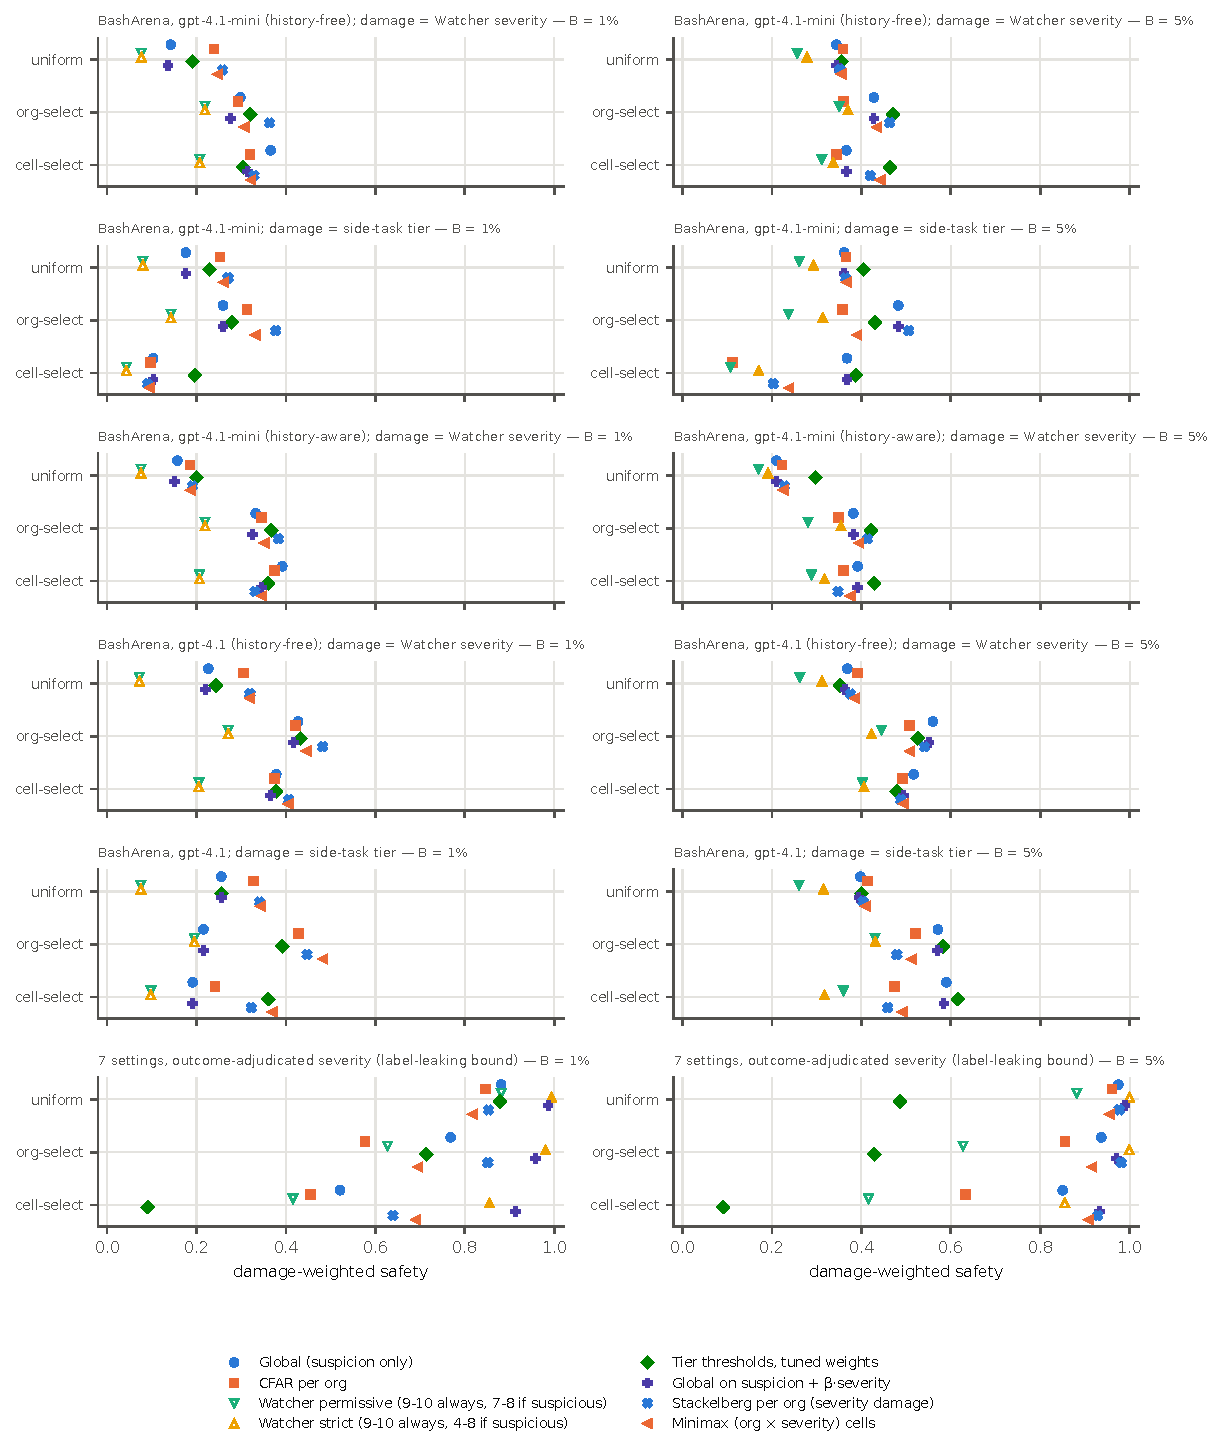
\includegraphics[width=0.6\linewidth]{r3_t2/figures/watcher_policies.pdf}
\caption{Round 3 policy comparison: damage-weighted safety against uniform, org-selecting and cell-selecting attackers. Only the 5\% panels are valid; the 1\% panels mix clamped replicates (audit2 m9). The bottom row (akshn\_adj) uses label-leaking severity. \src{r3_t2/figures/}}
\end{figure}

\section{What holds, what is weakened, what is dropped}\label{sec:verdicts}
\begingroup\footnotesize
\begin{xltabular}{\linewidth}{@{}>{\raggedright\arraybackslash}X>{\raggedright\arraybackslash}p{1.8cm}>{\raggedright\arraybackslash}p{4.4cm}@{}}
\toprule
Claim & Status & Evidence\\
\midrule
\endhead
Heterogeneity across deployments ($\tau$ 1.34--1.75), small within LinuxArena, none across agent models & \HOLD & \src{t2/tables.md}\\
White-box probe scores are far more context-dependent than LLM scores & \HOLD & honest-only; \src{fixes/corrections.csv (M5)}\\
CFAR is the worst rule against context selection (7 settings 1\%, ControlArena 5\%) & \HOLD & independent attacker info: \src{audit/repro_t2.csv}\\
A few alarm-feedback probes suffice to exploit CFAR; Stackelberg is flat & \HOLD & \src{r2_t2/tables.md (E4a)}\\
Stackelberg $>$ global against selection at 5\% (7 settings) & \HOLD & $+0.03..+0.12$; indep.\ info 0.957; \src{fixes/corrections.csv (m2)}\\
Stackelberg $>$ global against selection at 1\% (7 settings) & \WEAK & matched $[-0.11,+0.20]$\\
Stackelberg $>$ global at 1\% on ControlArena & \DROP & over-spend; matched 0.610 vs 0.607\\
Plug-in per-context quantiles over-spend with small $n$; Mondrian silent; pooled\_cv near budget & \HOLD & \src{t2/tables.md}\\
CFAR / max-detect raise uniform TPR for weak monitors (round 1, MB clusters) & \WEAK & rows partly clamped (m\_ok 0.34--0.70)\\
CFAR breaks at $\varepsilon\approx B$; global at $\varepsilon\approx B/w_t$ & \HOLD & \src{t2/tables.md}\\
OS-CFAR (LOCO) holds 0.77--0.86 under poisoning & \WEAK & per panel 0.62--0.81 at 10\%; worst target 0.07--0.45; \src{fixes/corrections.csv (m3)}\\
OS-CFAR (LOCO) as the recommended poisoning defense & \DROP & breaks under spread poisoning (E2)\\
Frozen-reference tail robust to spread poisoning, over-spends under deployment-wide tail drift & \HOLD & \src{r2_t2/tables.md (E2)}\\
Per-context thresholds do not transfer to a new agent; offsets + recalibrated level do & \HOLD & \src{r2_t2/tables.md (E1b)}\\
Stackelberg fit on other side tasks ``worse than global'' & \WEAK & significant vs in-distribution only\\
Cell severity minimax 0.92 / 0.95 vs global 0.64 / 0.71 & \WEAK & intervals touch or cross 0\\
E5: CFAR roughly doubles probe TPR at 1\% & \WEAK & 1\% \NE; 1.3--1.5$\times$ at equal spend; \src{fixes/corrections.csv (C1)}\\
E5: all 1\% spend-matched rows & \DROP & clamped; \src{fixes/corrections.csv (C1)}\\
E5: Stackelberg $\ge$ global on 14/17 signals at 5\% & \WEAK & 10/17 grouped, 0 CIs $>0$; \src{fixes/corrections.csv (M5)}\\
E5 AUROCs (gpt-4.1 0.911, \texttt{fibs\_fu\_full} 0.905, \ldots) & \WEAK & originals 0.45--0.83; fabrication confound\\
Blind severity does not separate (AUROC 0.53--0.54) & \HOLD & \src{r3_t2/tables.md}\\
Watcher tiers infeasible at 1\% and lose to global at 5\% & \HOLD & \src{audit2/issues.csv (m9)}\\
r3\_t2 1\% ``matched'' rows (per-org rules, tilt) & \DROP & clamped mixtures; \src{audit2/r3t2_matched_check.csv}\\
akshn\_adj severity results (0.98--0.99) & \WEAK & label-leaking upper bound; \src{fixes/corrections.csv (m11)}\\
\bottomrule
\end{xltabular}
\endgroup

\subsection{Errata relative to the October 21 version}
\begin{enumerate}
\item \textbf{Summary item 3 and the allocation table} (``Stackelberg 0.79 vs 0.64 at 1\%''): the 1\% gain is not established once spend-matched (interval $-0.11..+0.20$). The 5\% gain stands. With attacker information independent of the defender's fit the 1\% / 5\% values are 0.775 / 0.957, not 0.791 / 0.966.
\item \textbf{ControlArena 1\% Stackelberg row} (0.729, $-0.07..+0.27$): dropped. The nominal advantage is over-spending (1.38\% vs 0.97\%); spend-matched it is 0.610 vs 0.607, with only 66\% of replicates bracketed.
\item \textbf{Allocation caption} (``the spend-matched rows remove this; their conclusions are the same''): false for Stackelberg at 1\%, and the round-1 matcher clamps when its sweep misses $B$. Rows with \texttt{matched\_ok}$\,<0.8$ are now flagged.
\item \textbf{Weak-monitor bullet} (``nano trajectory at 5\%: 0.079 $\to$ 0.106 / 0.162''): these rows have \texttt{matched\_ok} 0.70 / 0.34 and max-detect realizes 5.56\%; the gain is not established.
\item \textbf{Summary item 5, poisoning table and recipe step 4} (``OS-CFAR with a LOCO tail holds 0.77--0.86 and still tracks genuine drift''; ``use OS-CFAR with a leave-one-context-out tail''): the range is one panel's; per panel 0.62--0.81 at $\varepsilon=10\%$ with worst targets at 0.07--0.45, and a clean-data cost on LA task category (0.778 vs 0.914). Under poisoning spread across contexts the LOCO tail breaks at $\varepsilon\approx B$ (worst 0.16--0.18 at 5\%). The recommended defense is now a frozen-reference tail with trusted refresh.
\item \textbf{``Untested: transfer across datasets; poisoning across several contexts''}: both were tested in round 2 (E1, E2).
\item \textbf{Recipe step 3} (``use Stackelberg fit on held-out attack data''): now conditional on attack data from the deployed side-task distribution and $\gtrsim$10--20 attacks per context or shrinkage (E1a, E4b).
\item \textbf{Spend line}: \$17.11 was round 1 only; the track total is \$38.93.
\item The October 21 version did not cover rounds 2--3. The round-2/3 log entries' E5 statements (``CFAR roughly doubles uniform TPR'', ``Stackelberg $\ge$ global on 14/17 signals'') are corrected in Section~5; the round-3 log's 1\% statements are limited to infeasibility.
\end{enumerate}

\section{Practitioner recipe}
\begin{enumerate}
\item \textbf{Measure before allocating.} Fit the random-effects $\tau$ on per-context exceedances of a global 5--10\% threshold, on honest data. If $\tau$ is not significant (LLM monitors within one deployment, LinuxArena, BashArena clusters), use one global threshold. Expect large $\tau$ for white-box probe signals and across deployments that share a monitor.
\item \textbf{Check budget feasibility.} Plug-in per-context thresholds cannot spend less than $\approx\sum_c w_c/(n_c+1)$. Do not run per-context quantiles when that floor exceeds $B$ (roughly $n_c\lesssim3/B$); use partial pooling with cross-validated $n_0$, which falls back to global. Always report realized spend next to any per-context TPR.
\item \textbf{If the attacker cannot choose its context} and the signal is heterogeneous (probes), per-context normalization raises detection at equal spend (\texttt{dec} probes $+0.18..+0.23$). Compare at equal realized spend, not at nominal level.
\item \textbf{If the attacker can choose its context, never use CFAR}: alarm feedback from 3--5 probes per context is enough to exploit it. Use Stackelberg (damage-equalizing) thresholds only with $\gtrsim$10--20 attacks per context from the deployed side-task distribution, or shrunk toward the pooled attacks ($m_0\approx10$, $\lambda\approx0.5$); otherwise use global. Use severity-weighted cell minimax only when per-cell damage is known.
\item \textbf{New agent model}: do not reuse per-context thresholds. Reuse the per-context offsets and recalibrate one global level on the new agent.
\item \textbf{Recalibration under a possible poisoner}: keep a frozen trusted reference; take per-context offsets from the new window and the tail from the reference; refresh the reference only through a trusted channel. Budget for 2--3$\times$ over-spend during genuine deployment-wide tail drift until the refresh. A LOCO tail is adequate only if the attacker can reach a single context. Outlier filters only slow a boiling frog.
\item \textbf{Expect within-context attack-type selection} to cost 0.2--0.4 more than allocation can recover.
\end{enumerate}

\subsection*{Recipe for a Watcher-like product (round 3)}
\begin{enumerate}
\item Rank actions by suspicion with one budget-matched threshold per deployment.
\item Do not hard-wire an always-block tier: measure its honest hit rate first (here 1.5\% of honest trajectories, above a 1\% budget).
\item Use severity as a tilt only if a validation set shows it discriminates; tune $\beta$ and accept $\beta\to0$.
\item Go per-org only after measuring org heterogeneity ($\tau$), and then with Stackelberg (with $\ge$20 attacks per org, or shrunk), never CFAR.
\item Expect white-box probe signals to need per-context normalization against uniform attackers, and pair it with damage-equalizing allocation against selection.
\end{enumerate}

\section{Limitations and open questions}
\begin{itemize}
\item \textbf{Monitor strength.} The Gemini panels are near-separable (AUROC $\approx0.99$); the MonitoringBench monitors are weak. Allocation effects are cleanest in between.
\item \textbf{Few attacks per context} in the LinuxArena sweep (5--18) and in E5 (6--42 base attacks per cluster), so attack-fitted rules (Stackelberg, max-detect) are noisy there.
\item \textbf{The spend matcher.} Round-1 and round-2 tables still use the clamping matcher; this report flags but does not re-estimate their \texttt{matched\_ok}$\,<0.8$ rows. Re-running them with the fixed matcher is cheap (no API cost).
\item \textbf{Attacker modeling.} The informed attacker uses its own calibration-split attacks; the oracle is biased low (winner's curse). Damage weights are synthetic except E3's adjudicated severity, which leaks the label.
\item \textbf{E5 confound.} 94\% of E5 attacks have LLM-fabricated tool outputs; probes may key on fabrication. Only 33 originals are clean, 1--15 per cluster.
\item \textbf{Severity rater.} One rater model (gpt-4.1-mini) and one prompt. A rater that sees the side task would leak the label like akshn\_adj.
\item \textbf{Open}: poisoning against Stackelberg's attack-data refits; a trusted-refresh protocol and its cadence; per-context allocation for white-box probes on clean (non-fabricated) attacks at scale.
\item \textbf{Negative results}: TM-CFAR is dominated; empirical-Bayes $n_0$ is worse than cross-validated $n_0$; agent model is not a useful context; side-task taxonomy weights are a poor damage proxy; severity tilt adds nothing with a blind rater.
\end{itemize}

\section*{Reproduction}
Code: \texttt{tracks/t2\_per\_context/} (round 1), \texttt{tracks/r2\_t2/} (round 2 and E5), \texttt{tracks/r3\_t2/} (round 3), \texttt{tracks/fixes/e5/} (C1 / M5 / m2 / m3 / m11 fixes), \texttt{tracks/audit2/} (second audit). Results: \texttt{results/t2/}, \texttt{results/r2\_t2/}, \texttt{results/r3\_t2/}, \texttt{results/fixes/\{t2,r2\_t2,r3\_t2\}/}, \texttt{results/audit/}, \texttt{results/audit2/}. Raw replicates: \texttt{data/processed/\{r2\_t2\_runs,r3\_t2\_runs\}/}. Narrative: \texttt{EXPERIMENT\_LOG.md} (entries ``T2 per-context thresholds'', ``T2 ROUND 2'', ``T2 ROUND 3'', ``Audit fixes'', ``Second-pass audit''). Repository: \url{https://github.com/gregkocher/agent-monitor-detection} (private).
\end{document}
